\section{Ideas}

Here I will approach three of the main ideas that integrated to form
the modern personal computer environment: Graphical user interface,
constructionism, and augmentative systems. \cite{smalltalk:kay_alan__early_history_smalltalk}

This division will at times seem artificial, not only because they
influenced each other, but because there is great overlapping of
techniques and philosophy between them. On the other hand this
structure does capture important distinctions and points of view that
are valuable to understand the whole story.

As with any history, there can be a great level of details, and all of
the ideas presented here have much more intricacies and were
implemented in a great deal of different systems. Most of this fine
grained idiosyncrasies will be left out because of my intention to
give a high level view of the subject. This subject was treated in a
more detailed and authoritative view by the references used here,
which the reader is encouraged to follow.

\subsection{GUI}

The development of all graphic environments can be traced directly to
Ivan Sutherland's sketchpad. Its ideas \emph{still influence how every
  computer user thinks about computing.}\cite{graphics:sutherland__sketchpad}

It did that by introducing graphic metaphors and devices, such as the
light-pen, the rubber band graphic manipulation, icons and a great
deal of the things most people take as ``natural'' when manipulating
modern GUI. \cite{graphics:sutherland__sketchpad}

But the major influence for programming paradigms was because its
object oriented features, which along with Simula \footnote{Both share
  a common ancestor in the work of Douglas T. Ross
  \cite{graphics:sutherland__sketchpad}} had a major impact in the
inspiration and development of Smalltalk: 

\begin{quote}
  What Simula was allocating were structures very much like the
  instances of Sketchpad. There were descriptions that acted like
  masters and they could create instances, each of which was an
  independent entity. What Sketchpad called masters and instances,
  Simula called activities and processes. ...

  This was the big hit, and I've not been the same since.
  \cite{smalltalk:kay_alan__early_history_smalltalk}
\end{quote} 




\subsection{Constructionism}

Programming is an activity that deals primarily with the construction
of abstract structures from ideas. This process and some of its encompassing
theories are usually neglected or just fade into the conceptual
background. This void is filled by constructionism, a learning theory
developed by Seymour Papert and his colleagues that:

\begin{quote}
  ... shares constructivism's connotation of learning as ``building
  knowledge structures'' irrespective of the circumstances of the
  learning. It then adds the idea that this happens especially
  felicitously in a context where the learner is consciously engaged in
  constructing a public entity, whether it's a sand castle on the beach
  or a theory of the universe.
  \cite{education:papert__situating_constructionism}
\end{quote}

The proponents of this theory were the front-runners of using
computers as a \emph{personal media}. They did that in order to
propose an alternative to instructionism and technocentrism. Those
ideas can be summarized in the claim that \emph{``To get better
  education, we must improve instruction. And if we're going to use
  computers, we'll make the computers do the
  instructon.''}. \cite{education:papert__constructionism_instructionism} 

Constructionism's alternative consists of using media, technology, and
social environments as scaffolds to the conceptual structures that is
to be built by people in the active role of their education. This
education was initially children learning math supported by
constructionism's answer to traditional math curricula, Logo. 

\begin{wrapfigure}{r}{40mm}
  \begin{center}
    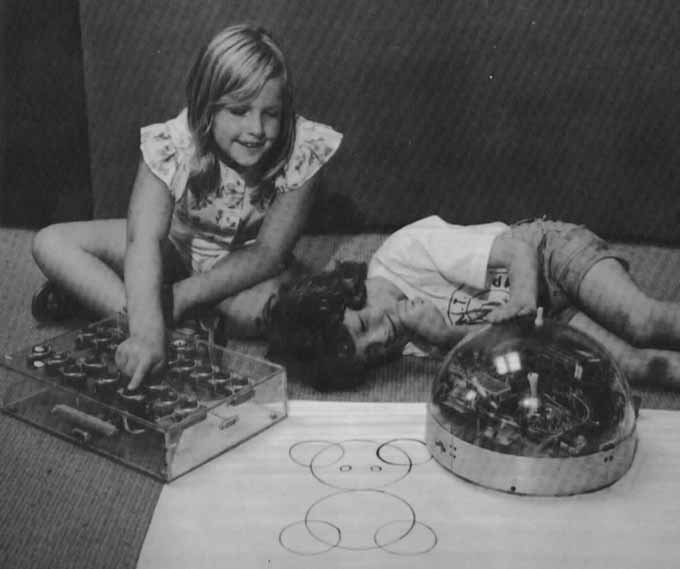
\includegraphics[scale=0.7]{images/mindstorms_turtle.jpg}
  \end{center}
  \caption{Children programming in logo. \cite{education:papert_mindstorms}}
\end{wrapfigure}

Logo profoundly influenced modern computer languages and environments
through the heavy impact it had on the development of the Smalltalk
system:

\begin{quotation}
  
  I finally visited Seymour Papert, Wally Feurzig, Cynthia Solomon and
  some of the other original researchers who had built LOGO and were
  using it with children in the Lexington schools. Here were children
  doing real programming with a specially designed language and
  environment. As with Simula's leading to OOP, this encounter finally
  hit me with what the destiny of personal computing really was going
  to be. Not a personal dynamic vehicle, as in Engelbart's metaphor
  opposed to the IBM ``railroads'', but something much more profound: a
  personal dynamic medium. With a vehicle one could wait until high
  school and give ``drivers ed'', but if it was a medium, it had to
  extend into the world of childhood. 
  \cite{smalltalk:kay_alan__early_history_smalltalk}

\end{quotation}

\section{Collaborative and Augmentative Systems}


\begin{wrapfigure}{r}{40mm}
  \begin{center}
    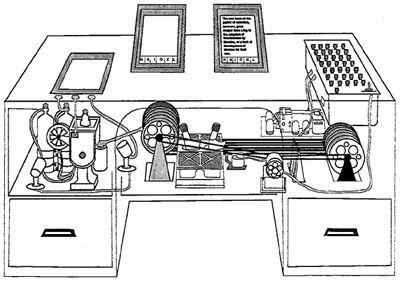
\includegraphics[scale=0.4]{images/memex.jpg}
  \end{center}
  \caption{ Memex, as it was illustrated for LIFE Magazine, 1945. The
    desk contains two main microfilm projectors and mechanical
    apparatus to retrieve the pages for a given
    trail. \cite{hypertext:muller__vision_and_reality}}
\end{wrapfigure}

Users nowadays use several metaphors for networked computers, such as
links, bookmarks, hypertext, web, publishing, collaborative editing
and so forth. These concepts seem ``natural'', but they are as
artificial as the tools that embody them. We can trace their creation
to their modern creator, Vannevar
Bush. \footnote{ Bush as responsible for a great deal more, such as being the man
responsible for the creation of the modern american military-scientific
establishment. \cite{history:pascal__godfather} } Bush, in his highly
influential 1945 article \cite{hypertext:bush__as_we_may_think}
elaborated about the memex, which had a stark similarity with the
modern personal computer and the internet:

\begin{quotation}
  The owner of the memex, let us say, is interested in the origin and
  properties of the bow and arrow. Specifically he is studying why the
  short Turkish bow was apparently superior to the English long bow in
  the skirmishes of the Crusades. He has dozens of possibly pertinent
  books and articles in his memex. First he runs through an
  encyclopedia, finds an interesting but sketchy article, leaves it
  projected. Next, in a history, he finds another pertinent item, and
  ties the two together. Thus he goes, building a trail of many
  items. Occasionally he inserts a comment of his own, either linking
  it into the main trail or joining it by a side trail to a particular
  item. When it becomes evident that the elastic properties of
  available materials had a great deal to do with the bow, he branches
  off on a side trail which takes him through textbooks on elasticity
  and tables of physical constants. He inserts a page of longhand
  analysis of his own. Thus he builds a trail of his interest through
  the maze of materials available to him. 
\end{quotation}


\begin{wrapfigure}{r}{40mm}
  \begin{center}
    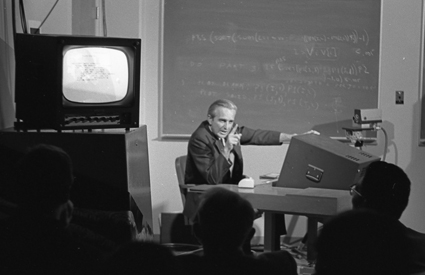
\includegraphics[scale=0.4]{images/engelbart-demo.jpg}
  \end{center}
  \caption{Engelbart demo, 1968.}
\end{wrapfigure}

But if Bush was the original thinker, the original builder was Douglas
Engelbart. His efforts resulted in \emph{Not just hypertext, but
  graphics, multiple panes, efficient navigation and command input,
  interactive collaborative work, etc. An entire conceptual world and
  world view }\cite{smalltalk:kay_alan__early_history_smalltalk}
\cite{intelligence:engelbart__augmenting}.

Engelbart's 1968 demonstration took place in the American Federation of
Information Processing Societies' Fall Joint Computer Conference. It
shook the world then, and it when on the have an enormous amount of
influence in the community that created the personal computer
revolution. \cite{hypertext:muller__vision_and_reality}

\begin{quote}
  The impact of this vision was to produce in the minds of those who
  were ``eager to be augmented'' a compelling metaphor of what
  interactive computing should be like, and I immediately adopted many
  of the ideas for the FLEX machine. 
  \cite{smalltalk:kay_alan__early_history_smalltalk}
\end{quote}


